%%%%%%%%%%%%%%%%%%%%%%%%%%%%%%%%%%%%%%%%%
% Jacobs Landscape Poster
% LaTeX Template
% Version 1.0 (29/03/13)
%
% Created by:
% Computational Physics and Biophysics Group, Jacobs University
% https://teamwork.jacobs-university.de:8443/confluence/display/CoPandBiG/LaTeX+Poster
% 
% Further modified by:
% Nathaniel Johnston (nathaniel@njohnston.ca)
%
% This template has been downloaded from:
% http://www.LaTeXTemplates.com
%
% License:
% CC BY-NC-SA 3.0 (http://creativecommons.org/licenses/by-nc-sa/3.0/)
%
%%%%%%%%%%%%%%%%%%%%%%%%%%%%%%%%%%%%%%%%%

%----------------------------------------------------------------------------------------
%	PACKAGES AND OTHER DOCUMENT CONFIGURATIONS
%----------------------------------------------------------------------------------------

\documentclass[24pt,final]{beamer}


\usepackage[scale=0.95]{beamerposter} % Use the beamerposter package for laying out the poster

%%%%%%%%%%%%%%%%%%
%%%%%%%%%%%%%%%%%%
%%%%%%%%%%%%%%%%%%
%% shaded theorems
%%%%%%%%%%%%%%%%%%
%%%%%%%%%%%%%%%%%%
%%%%%%%%%%%%%%%%%%


\usepackage{mdframed} 
\usepackage{thmtools}

%\newtheoremstyle{selfdefined}
%{12pt}% Space above
%{12pt}% Space below
%{}% Body font \itshape =italian style 
%{}% Indent amount
%{\bfseries}% Theorem head font
%{}% Punctuation after theorem heading
%{\newline}% Space after theorem heading, 0.5em => in gleicher zeile weiter
%{}% Theorem head spec (can be left empty, meaning ‘normal’)

\definecolor{shadecolor}{gray}{0.95}
\declaretheoremstyle[
headfont=\normalfont\bfseries,
notefont=\mdseries, notebraces={(}{)},
bodyfont=\normalfont,
postheadspace=0.5em,
spaceabove=1pt,
mdframed={
  skipabove=8pt,
  skipbelow=8pt,
  hidealllines=true,
  backgroundcolor={shadecolor},
  innerleftmargin=4pt,
  innerrightmargin=4pt}
]{shaded}




\usepackage[colorinlistoftodos,bordercolor=orange,backgroundcolor=orange!20,linecolor=orange,textsize=scriptsize]{todonotes}
%\renewbibmacro{in:}{\ifentrytype{article}{}{\printtext{\bibstring{in}\intitlepunct}}} % don't print "in" for articles



\graphicspath{{../figures/}}  % Path to figures folder
\newcommand{\R}{\mathbb{R}}
\newcommand{\C}{\mathbb{C}}
\newcommand{\N}{\mathbb{N}}
\newcommand{\K}{\mathcal{K}}
\newcommand{\A}{\mathcal{A}}
\newcommand{\bH}{\mathbf{H}}
    
  \newcommand{\argmin}{\text{\rm argmin}}
\newcommand{\eqdef}{\; { := }\;}
\providecommand{\Null}[1]{\mathbf{Null}\left( #1\right)}
\providecommand{\Rank}[1]{\mathbf{Rank}\left( #1\right)}
\providecommand{\rank}[1]{\mathbf{Rank}\left( #1\right)}
\providecommand{\Range}[1]{\mathbf{Range}\left( #1\right)}
\providecommand{\range}[1]{\mathbf{Range}\left( #1\right)}
\providecommand{\Tr}[1]{\mathbf{Tr}\left( #1\right)}
\providecommand{\trace}[1]{\mathbf{Tr}\left( #1\right)}
\providecommand{\diag}[1]{\mathbf{Diag}\left( #1\right)}
\providecommand{\E}[1]{\mathbb{E}\left[ #1\right]}
% \providecommand{\EE}[2]{\mathbb{E}_{#1}\left[ #2\right]}
\newcommand{\EE}{\mathbb{E}}
\providecommand{\Prob}[1]{\mathbb{P}\left[ #1\right]}
  \providecommand{\dotprod}[1]{\langle #1\rangle} 
\providecommand{\norm}[1]{\lVert#1\rVert}
\providecommand{\colvec}[1]{{\text{\scriptsize $
\begin{array}{c}
 #1
\end{array}$
}}}



\newcommand{\rob}[1]{\todo[inline]{\textbf{Robert: }#1}}
\newcommand{\pet}[1]{\todo[inline]{\textbf{Peter: }#1}}
\newcommand{\filip}[1]{\todo[inline]{\textbf{Filip: }#1}}
\newcommand{\seb}[1]{\todo[inline]{\textbf{Sebastian: }#1}}


\newcommand{\cA}{{\mathcal A}}
\newcommand{\cB}{{\mathcal B}}
\newcommand{\cC}{{\mathcal C}}
\newcommand{\cD}{{\mathcal D}}
\newcommand{\cE}{{\mathcal E}}
\newcommand{\cF}{{\mathcal F}}
\newcommand{\cG}{{\mathcal G}}
\newcommand{\cH}{{\mathcal H}}
\newcommand{\cJ}{{\mathcal J}}
\newcommand{\cK}{{\mathcal K}}
\newcommand{\cL}{{\mathcal L}}
\newcommand{\cM}{{\mathcal M}}
\newcommand{\cN}{{\mathcal N}}
\newcommand{\cO}{{\mathcal O}}
\newcommand{\cP}{{\mathcal P}}
\newcommand{\cQ}{{\mathcal Q}}
\newcommand{\cR}{{\mathcal R}}
\newcommand{\cS}{{\mathcal S}}
\newcommand{\cT}{{\mathcal T}}
\newcommand{\cU}{{\mathcal U}}
\newcommand{\cV}{{\mathcal V}}
\newcommand{\cX}{{\mathcal X}}
\newcommand{\cY}{{\mathcal Y}}
\newcommand{\cW}{{\mathcal W}}
\newcommand{\cZ}{{\mathcal Z}}




% matrices
%\newcommand{\mA}{{ A}}
%\newcommand{\mB}{{ B}}
%\newcommand{\mC}{{ C}}
%\newcommand{\mD}{{ D}}
%\newcommand{\mE}{{ E}}
%\newcommand{\mF}{{ F}}
%\newcommand{\mG}{{ G}}
%\newcommand{\mH}{{ H}}
%\newcommand{\mI}{{I}}
%\newcommand{\mJ}{{ J}}
%\newcommand{\mK}{{ K}}
%\newcommand{\mL}{{ L}}
%\newcommand{\mM}{{ M}}
%\newcommand{\mN}{{ N}}
%\newcommand{\mO}{{ O}}
%\newcommand{\mP}{{ P}}
%\newcommand{\mQ}{{ Q}}
%\newcommand{\mR}{{ R}}
%\newcommand{\mS}{{ S}}
%\newcommand{\mT}{{ T}}
%\newcommand{\mU}{{ U}}
%\newcommand{\mV}{{ V}}
%\newcommand{\mW}{{ W}}
%\newcommand{\mX}{{X}}
%\newcommand{\mY}{{ Y}}
%\newcommand{\mZ}{{ Z}}
%\newcommand{\mLambda}{{ \Lambda}}

\newcommand{\bigZ}{{ \mathbf{Z}}}

\newcommand{\gS}{ {\mS_0}}


%Vectorization
\providecommand{\Vect}[1]{\mathbf{Vec}\left( #1\right)}
\providecommand{\invVec}[1]{\mathbf{Vec^{-1}}\left( #1\right)}
\newcommand{\vX}{{X_{\text{v}}}}
\newcommand{\vI}{{I_{\text{v}}}}

%ef21: new commands

\newcommand {\maxin}{\max_{i=1,\dots, n}}
\newcommand {\maxi}{\max_{i}}
\newcommand {\minin}{\min_{i=1,\dots, n}}
\newcommand {\mini}{\min_{i}}
\newcommand {\sumin}{\sum_{i=1}^{n}}
\newcommand {\suminn}{\fr{1}{n}\sum_{i=1}^{n}}
\newcommand {\sumjm}{\sum_{j=1}^{m}}
\newcommand {\sumjmi}{\sum_{j=1}^{m_i}}
\newcommand {\sumjmm}{\fr{1}{m}\sum_{j=1}^{m}}
\newcommand {\sumjnn}{\fr{1}{n}\sum_{j=1}^{n}}
\newcommand {\sumjmmi}{\fr{1}{m_i}\sum_{j=1}^{m_i}}
\newcommand {\sumjn}{\sum_{j=1}^{n}}
\newcommand {\wik}{w_{i}^{k}}
\newcommand {\wjk}{w_{j}^{k}}
\newcommand {\wk}{w^{k}}
\newcommand {\wikpo}{w_{i}^{k+1}}
\newcommand {\wjkpo}{w_{j}^{k+1}}
%\newcommand {\sumin}{\sum_{i=1}^{n}}
\newcommand {\sumid}{\sum_{i=1}^{d}}
\newcommand {\ghx}{\hat{g}(x)}
\newcommand {\gh}{\hat{g}}
\newcommand {\gih}{\hat_i}
\newcommand {\gihx}{\hat{g_i}(x)}
%\newcommand {\sumjn}{\sum_{j=1}^{n}}
\newcommand{\cmark}{\textcolor{blue}{\ding{51}}}%
\newcommand{\xmark}{\textcolor{red}{\ding{55}}}%

\newcommand{\lamax}[1]{\lam_{\max}\left(#1\right)}
\newcommand{\lamin}[1]{\lam_{\min}\left(#1\right)}
\newcommand{\rb}[1]{\left(#1\right)}
\renewcommand{\sb}[1]{\left[#1\right]}
\newcommand{\cb}[1]{\lt\{#1\rt\}}

\newcommand {\rbl}[1]{(#1)} %round braces without left - right alignment
%\renewcommand{\nf}[1]{\nabla f\rbl{#1}}
\newcommand{\nfi}[1]{\nabla f_i\rbl{#1}}
\newcommand{\nfj}[1]{\nabla f_j\rbl{#1}}

\newcommand{\xk}{x^{k}}
\newcommand{\xt}{x^{t}}
\newcommand{\xtpo}{x^{t+1}}
\newcommand{\xkpo}{x^{k+1}}
\newcommand{\fxk}{f(\xk)}
\newcommand{\gxk}{g(\xk)}
\newcommand{\fxkpo}{f(\xkpo)}
\newcommand{\dz}{\delta_0}
\newcommand{\xs}{x^{\star}}
\newcommand{\nfxk}{\nf{\xk}}
\newcommand{\nfxkpo}{\nf{x^{k+1}}}
\newcommand{\nfxt}{\nf{\xt}}
\newcommand{\nfxtpo}{\nf{\xtpo}}
\newcommand{\nfomt}{\nf{\omt}}
\newcommand{\nfomtpo}{\nf{\omtpo}}
\newcommand{\nfxs}{\nf{\xs}}
\newcommand{\nfx}{\nf{x}}
\newcommand{\nfy}{\nf{y}}
\newcommand{\nfxijk}{\nabla f_{\xi_{ij}^k} (x^k)}
\newcommand{\nfxijkpo}{\nabla f_{\xi_{ij}^k}(x^{k+1})}
\newcommand{\nfixk}{\nfi{\xk}}
\newcommand{\nfixt}{\nfi{\xt}}
\newcommand{\nfix}{\nfi{x}}
\newcommand{\nfiy}{\nfi{y}}
\newcommand{\nfijx}{\nabla f_{ij}(x)}
\newcommand{\nfijy}{\nabla f_{ij}(y)}
\newcommand{\dgt}{\Delta g^{t}}
\newcommand{\dgtpo}{\Delta g^{t+1}}
\newcommand{\gt}{ g^{t}}
\newcommand{\gtpo}{ g^{t+1}}

\newcommand{\dgit}{\Delta g_i^{t}}
\newcommand{\dgitpo}{\Delta g_i^{t+1}}

\newcommand{\omitpo}{\omega_i^{t+1}}
% \renewcommand{\omit}{\omega_i^{t}}

\newcommand{\nfiomtpo}{\nfi{\omitpo}}
\newcommand{\nfitpoxtpo}{\nabla f_{i_{t+1}}(x^{t+1})}

%\newcommand{\nfix}{\nfi{x}}

\newcommand{\nfixs}{\nfi{\xs}}
\newcommand{\nfjxk}{\nfj{\xk}}
\newcommand{\nfjxs}{\nfj{\xs}}
\newcommand{\nfixkpo}{\nfi{x^{k+1}}}
\newcommand{\nfixtpo}{\nfi{x^{t+1}}}
\newcommand{\nfitxt}{\nabla f_{i_{t}}(x^{t})}
\newcommand{\nfitomt}{\nabla f_{i_{t}}(\omt)}
%\newcommand{\nfitpoxtpo}{\nabla f_{i_{t+1}}(x^{t+1})}
\newcommand{\nfitpoomtpo}{\nabla f_{i_{t+1}}(\omtpo)}

\newcommand{\nfjxkpo}{\nfj{x^{k+1}}}
\newcommand{\hik}{h^{k}_{i}}
\newcommand{\ali}{\al_{i}}
\newcommand{\mik}{m^{k}_{i}}
\newcommand{\hikpo}{h^{k+1}_{i}}
\newcommand{\hk}{h^{k}}
\newcommand{\nmo}{\fr{1}{n}}
\newcommand{\nmt}{\fr{1}{n^2}}
\newcommand{\tnmo}{\fr{2}{n}}
\newcommand{\tnmt}{\fr{2}{n^2}}
\newcommand{\ub}{\underbrace}
\newcommand{\omi}{\omega_i}
\newcommand{\om}{\omega}
\newcommand{\omtpo}{\omega^{t+1}}
\newcommand{\omt}{\omega^{t}}

\newcommand{\z}{\zeta}
\newcommand{\lt}{\left}
\newcommand{\rt}{\right}
\newcommand{\al}{\alpha}
\newcommand{\p}{\partial}
\newcommand{\D}{\Delta}
\newcommand{\fr}{\frac}
\newcommand{\dfr}{\dfrac}
\newcommand{\mbf}{\mathbf}
\newcommand{\mds}{\mathds}
\newcommand{\bb}{\mathbb}
\newcommand{\wt}{\widetilde}
\newcommand{\wS}{\wt{S}}
\newcommand{\wA}{\wt{A}}
\newcommand{\wL}{\wt{L}}
\newcommand{\wB}{\wt{B}}
\newcommand{\wC}{\wt{C}}
\newcommand{\ws}{\wt{s}}
\newcommand{\wg}{\wt{g}}
\newcommand{\wgix}{\wg_i(x)}
\newcommand{\wgiy}{\wg_i(y)}
\newcommand{\wgik}{\wg_i(x^k)}
\newcommand{\wgikpo}{\wg_i(x^{k+1})}
\newcommand{\wgu}{\wt{g}^u}
\newcommand{\wG}{\wt{G}}
\newcommand{\hG}{\hat{G}}
\newcommand{\pA}{A^{\prime}}
\newcommand{\pB}{B^{\prime}}
\newcommand{\pC}{C^{\prime}}
\newcommand{\wpA}{\wA^{\prime}}
\newcommand{\wpB}{\wB^{\prime}}
\newcommand{\wpC}{\wC^{\prime}}
\newcommand{\ppA}{A^{\prime \prime}}
\newcommand{\ppB}{B^{\prime \prime}}
\newcommand{\ppC}{C^{\prime \prime}}


\newcommand{\hg}{\hat{g}}
\newcommand{\hgi}{\hat{g}_i}
\newcommand{\hgix}{\hat{g}_i(x)}
\newcommand{\hgiy}{\hat{g}_i(y)}
\newcommand{\hgik}{\hat{g}_i(x^k)}
\newcommand{\hgikpo}{\hat{g}_i(x^{k+1})}
\newcommand{\hgu}{\hat{g}^u}
\newcommand{\hs}{\hat{s}}


\newcommand{\eik}{e_i^t}
\newcommand{\gik}{g_i^t}
\newcommand{\gikpo}{g_i^{t+1}}
\newcommand{\eikpo}{e_i^{t+1}}
\newcommand{\vik}{v_i^t}
\newcommand{\vikpo}{v_i^{t+1}}

\newcommand{\git}{g_i^t}
\newcommand{\gitpo}{g_i^{t+1}}
\newcommand{\eit}{e_i^t}
\newcommand{\eitpo}{e_i^{t+1}}
\newcommand{\vit}{v_i^t}
\newcommand{\vitpo}{v_i^{t+1}}

\newcommand{\wcC}{\wt{\cC}}
\newcommand{\La}{\Lambda}
\newcommand{\lam}{\lambda}
\newcommand{\opn}{\operatorname}
\newcommand{\vp}{\varphi}
\newcommand{\bM}{\mbf M}
\newcommand{\bG}{\mbf G}
\newcommand{\bI}{\mbf I}
\newcommand{\bD}{\mbf D}
\newcommand{\bA}{\mbf A}
\newcommand{\bC}{\mbf C}
\newcommand{\bP}{\mbf P}
\newcommand{\bB}{\bb B}
\newcommand{\bU}{\bb U}
\newcommand{\bLa}{\mbf {\La}}
%\newcommand{\R}{\bb R}
\newcommand{\bE}{\mbf E}
\newcommand{\hS}{\hat{S}}
\newcommand{\eps}{{\varepsilon}}
\newcommand{\bL}{\mathbf{L}}
\newcommand{\stepsize}{\eta}
%\newcommand{\cE}{{\cal E}}
%\newcommand{\norm}[1]{\left\| #1 \right\|}
\newcommand{\lin}[1]{\left\langle #1\right\rangle} % product
%\newcommand{\cD}{\mathcal{D}}
%\newcommand{\cC}{\mathcal{C}}
%\newcommand{\cQ}{\mathcal{Q}}
\newcommand{\cCw}{\cC_{\omega}}
\newcommand{\cCd}{\cC_{\delta}}
\newcommand{\Ctk}[1]{\cC_{Tk}\rb{#1}}
\newcommand{\gixk}{g_{i}(x_k)}
%\newcommand{\cS}{\mathcal{S}}
\newcommand{\mM}{\mathbf{M}}
\newcommand{\mN}{\mathbf{N}}
\newcommand{\bN}{\mathbf{N}}
%\newcommand{\mI}{\mathbf{I}}
\newcommand{\mL}{\mathbf{L}}
\newcommand{\mD}{\mathbf{D}}
\newcommand{\bx}{\bar{x}}
\newcommand{\by}{\bar{y}}

\newcommand{\eqtext}[1]{\ensuremath{\stackrel{\text{#1}}{=}}}
\newcommand{\letext}[1]{\ensuremath{\stackrel{\text{#1}}{\le}}}
\newcommand{\getext}[1]{\ensuremath{\stackrel{\text{#1}}{\ge}}}
\newcommand{\succtext}[1]{\ensuremath{\stackrel{\text{#1}}{\succ}}}
\newcommand{\preceqtext}[1]{\ensuremath{\stackrel{\text{#1}}{\preceq}}}
\newcommand{\onenorm}[1]{\left\| #1 \right\|_1}      % norm 
\newcommand{\twonorm}[1]{\left\| #1 \right\|_2}      % norm 
\newcommand{\threenorm}[1]{\left\| #1 \right\|_3}      % norm 
\newcommand{\gnorm}[1]{\left\| #1 \right\|^{1 + \gamma }}      % norm 
\newcommand{\sqnorm}[1]{\left\| #1 \right\|^{2}}
\newcommand{\anorm}[1]{\left\| #1 \right\|^{\al}}      % norm 
\newcommand{\bnorm}[1]{\left\| #1 \right\|^{\beta}}      % norm 
\newcommand{\ahnorm}[1]{\left\| #1 \right\|^{\al/2}}      % norm 
\newcommand{\bbone}[1]{\mathbb{1}}      % norm 
\newcommand{\g}{\gamma}

%\newcommand{\nf}[1]{\nabla f\rb{#1}}      % norm 

\newcommand{\hotidea}{{\color{red}\bf HOT IDEA: }}
\newcommand{\done}{{\color{blue}\bf DONE: }}
%\newcommand{\cO}{{\cal O}}

\newcommand{\del}[1]{}

\newcommand{\finf}{f^\mathrm{inf}}
\newcommand{\fiinf}{f_i^\mathrm{inf}}

\let\la=\langle
\let\ra=\rangle

\def\<{\left\langle}
\def\>{\right\rangle}
% \def\[{\left[}
%\def\]{\right]}
\def\({\left(}
\def\){\right)}

%\newcommand{\st}{\;:\;}
\newcommand{\ve}[2]{\langle #1 ,  #2 \rangle}

%\newcommand{\eqdef}{\stackrel{\text{def}}{=}}

\newcommand{\ii}{{}^{(i)}}


%\newcommand{\Prob}{\mathbf{Prob}}
%\newcommand{\E}{\mathbf{E}}

%\usepackage{bbm}
%\usepackage{dsfont}

\newcommand{\vc}[2]{#1^{(#2)}}
\newcommand{\nc}[2]{{\color{red}\|#1\|_{(#2)}}}
\newcommand{\ncs}[2]{\|#1\|^2_{(#2)}}
\newcommand{\ncc}[2]{{\color{red}\|#1\|^*_{(#2)}}}
\newcommand{\ls}[1]{{\color{red} \mathcal S(#1)}}
\newcommand{\Rw}[2]{\mathcal R_{#1}(#2)}
\newcommand{\Rws}[2]{\mathcal R^2_{#1}(#2)}
\newcommand{\nbp}[2]{\|#1\|_{(#2)}}   % norm block primal
\newcommand{\nbd}[2]{\|#1\|_{(#2)}^*} % norm block dual
\newcommand{\lf}{\mathcal L}
\newcommand{\U}{U}
%\newcommand{\N}{N}
\newcommand{\mLi}{{\color{red}m^{(i)}}}
\newcommand{\gLi}{{\color{red}f{(i)}}}
%\newcommand{\TLi}{{\color{red}T_L^{(i)}}}
\newcommand{\TLi}[1]{{\color{blue}T^{(#1)}}}

\newcommand{\Lip}{L}

\newcommand{\Rc}[1]{{\color{red}  \mathbf{RC}_{(#1)}}}
\newcommand{\NRCDM}{{\color{red}NRCDM}\  }
\newcommand{\nnz}[1]{{\color{red}\|#1\|_0}}
% sets
\DeclareMathOperator{\card}{card}       % cardinality of a set
\DeclareMathOperator{\diam}{diam}       % diameter of a set
\DeclareMathOperator{\MVEE}{MVEE}       % minim volume enclosing ellipsoid of a set
\DeclareMathOperator{\vol}{vol}         % volume of a set

% statistical
% \DeclareMathOperator{\Exp}{{\rm E}}           % expectation
%\newcommand{\Exp}[1]{{\rm E}\left[#1\right]}
\newcommand{\Exp}[1]{{\bb E}\left[#1\right]}
\newcommand{\Expu}[2]{{\bb E}_{#1}\left[#2\right]}

\DeclareMathOperator{\Cov}{Cov}         % covariance
\DeclareMathOperator{\Var}{Var}         % variance
\DeclareMathOperator{\Corr}{Corr}       % correlation

% functions and operators
\DeclareMathOperator{\signum}{sign}     % signum/sign of a scalar
\DeclareMathOperator{\dom}{dom}         % domain
\DeclareMathOperator{\epi}{epi}         % epigraph
\DeclareMathOperator{\Ker}{null}        % nullspace/kernel
\DeclareMathOperator{\nullspace}{null}  % nullpsace
%\DeclareMathOperator{\range}{range}     % range
\DeclareMathOperator{\Image}{Im}        % image

% topology
\DeclareMathOperator{\interior}{int}    % interior
\DeclareMathOperator{\ri}{rint}         % relative interior
\DeclareMathOperator{\rint}{rint}       % relative interior
\DeclareMathOperator{\bdry}{bdry}       % boundary
\DeclareMathOperator{\cl}{cl}           % closure

% vectors, matrices
\DeclareMathOperator{\linspan}{span}
\DeclareMathOperator{\linspace}{linspace}
\DeclareMathOperator{\cone}{cone}

%\DeclareMathOperator{\tr}{tr}           % trace
%\DeclareMathOperator{\rank}{rank}       % rank
\DeclareMathOperator{\conv}{conv}       % convex hull
\DeclareMathOperator{\Diag}{Diag}       % Diag(v) = diagonal matrix with v_i on the diagonal
%\DeclareMathOperator{\diag}{diag}       % diag(D) = the diagonal vector of matrix D

\DeclareMathOperator{\Arg}{Arg}         % Argument

%\renewcommand{\qedsymbol}{\ding{114}}

%\newcommand{\lamax}[1]{\lam_{\max}\left(#1\right)}
%\newcommand{\lamin}[1]{\lam_{\min}\left(#1\right)}
%\newcommand{\rb}[1]{\left(#1\right)}
\renewcommand{\sb}[1]{\left[#1\right]}
%\newcommand{\cb}[1]{\lt\{#1\rt\}}

%\newcommand {\rbl}[1]{(#1)} %round braces without left - right alignment
%\renewcommand{\nf}[1]{\nabla f\rbl{#1}}
%\newcommand{\nfi}[1]{\nabla f_i\rbl{#1}}
%\newcommand{\nfj}[1]{\nabla f_j\rbl{#1}}

\usepackage{hyperref}
\hypersetup{
colorlinks=true,
linkcolor=red,
filecolor=red,
citecolor = black,
urlcolor=blue,
}

\usepackage{color, colortbl}
%\usepackage[abs]{overpic}
\usepackage{xcolor,varwidth}
\usepackage{enumitem}
\usepackage{adjustbox}

\usepackage{mdframed} 
\usepackage{thmtools}

\usepackage{makecell}

\usepackage[flushleft]{threeparttable} % http://ctan.org/pkg/threeparttable

\usepackage{caption}
\usepackage{multirow}
\usepackage{colortbl}
\definecolor{bgcolor}{rgb}{0.8,1,1}
\definecolor{bgcolor2}{rgb}{0.8,1,0.8}
\definecolor{niceblue}{rgb}{0.0,0.19,0.56}

\usetheme{confposter} % Use the confposter theme supplied with this template

\setbeamercolor{block title}{fg=ngreen,bg=white} % Colors of the block titles
\setbeamercolor{block body}{fg=black,bg=white} % Colors of the body of blocks
\setbeamercolor{block alerted title}{fg=white,bg=dblue!70} % Colors of the highlighted block titles
\setbeamercolor{block alerted body}{fg=black,bg=dblue!10} % Colors of the body of highlighted blocks

\setbeamercolor*{block title example}{fg=ngreen,
bg= white}
\setbeamercolor*{block body example}{fg=black,bg= green!5}

\usepackage{lipsum,lmodern}
\usepackage{tikz}
\usetikzlibrary{arrows.meta,arrows}
\usetikzlibrary{positioning}
\newcommand{\tikzcircle}[2][red,fill=red]{\tikz[baseline=-0.5ex]\draw[#1,radius=#2] (0,0) circle ;}
\usepackage[most]{tcolorbox}

\definecolor{GreyBlue}{rgb}{0.6,0.85,0.9}


% Many more colors are available for use in beamerthemeconfposter.sty
%\setbeamercolor{block example title}{fg=ngreen,bg=green!10} % Colors of the block titles
%\setbeamercolor{block example body}{fg=black,bg=green!10} % Colors of the body of blocks
%-----------------------------------------------------------
% Define the column widths and overall poster size
% To set effective sepwid, onecolwid and twocolwid values, first choose how many columns you want and how much separation you want between columns
% In this template, the separation width chosen is 0.024 of the paper width and a 4-column layout
% onecolwid should therefore be (1-(# of columns+1)*sepwid)/# of columns e.g. (1-(4+1)*0.024)/4 = 0.22
% Set twocolwid to be (2*onecolwid)+sepwid = 0.464
% Set threecolwid to be (3*onecolwid)+2*sepwid = 0.708

\newlength{\sepwid}
\newlength{\onecolwid}
\newlength{\twocolwid}
\newlength{\threecolwid}
\newlength{\fourcolwid}
\setlength{\paperwidth}{48in} % A0 width: 46.8in
\setlength{\paperheight}{36in} % A0 height: 33.1in
\setlength{\sepwid}{0.024\paperwidth} % Separation width (white space) between columns
\setlength{\onecolwid}{0.22\paperwidth} % Width of one column
\setlength{\twocolwid}{0.464\paperwidth} % Width of two columns
\setlength{\threecolwid}{0.708\paperwidth} % Width of three columns
\setlength{\fourcolwid}{0.928\paperwidth} % Width of three columns
\setlength{\topmargin}{-0.5in} % Reduce the top margin size
%-----------------------------------------------------------

\usepackage{graphicx}  % Required for including images

\usepackage{booktabs} % Top and bottom rules for tables

\usepackage{amssymb,amsmath,amscd,amsfonts,amstext,amsthm,bbm, enumerate, dsfont, mathtools}

\definecolor{cadmiumorange}{rgb}{0.93, 0.53, 0.18}
% \usepackage[lined, ruled]{algorithm2e}
% \usepackage{algpseudocode} 
% \usepackage{algorithmicx}

\usepackage{algorithm}
\usepackage{algorithmic}

\usepackage{array}

\usepackage{exscale}
\usepackage{nicefrac}
\usepackage{graphicx} % more modern
%\usepackage{subfigure} 
\usepackage{tcolorbox}
\tcbuselibrary{skins, theorems}
\tcbset{fonttitle=\footnotesize}

\definecolor{carrotorange}{rgb}{0.93, 0.68, 0.13}

\newcommand{\mA}{\mathbf{A}}
\newcommand{\mB}{\mathbf{B}}
\newcommand{\mC}{\mathbf{C}}
\newcommand{\mH}{\mathbf{H}}
\newcommand{\mI}{\mathbf{I}}
\newcommand{\mU}{\mathbf{U}}
\newcommand{\mZ}{\mathbf{Z}}

\newcommand{\NN}{\mathbb{N}}

\newcommand{\squeeze}{}

%\newcommand{\algname}[1]{{{\sf \footnotesize \color{red} #1}}\xspace}
\newcommand{\algname}[1]{{{\sf  #1}}}

\definecolor{mydarkgreen}{RGB}{39,130,67}
\definecolor{mydarkred}{RGB}{192,47,25}
\definecolor{mydarkblue}{RGB}{39,47,180}
\newcommand{\green}{\color{mydarkgreen}}
\newcommand{\red}{\color{mydarkred}}
\newcommand{\blue}{\color{mydarkblue}}

\newcommand{\thetaNEW}{{\red A}}
\newcommand{\betaNEW}{{\red B}}
\newcommand{\alphaNEW}{{\green\alpha}}
\newcommand{\lambdaNEW}{\alpha}

\usepackage{pifont}
% \newcommand{\cmark}{\text{\ding{51}}}
% \newcommand{\xmark}{\text{\ding{55}}}

%----------------------------------------------------------------------------------------
%	CUSTOM 
%----------------------------------------------------------------------------------------

%\newtheorem{proposition}{Proposition}

\usepackage[absolute,overlay]{textpos}
%\TPoptions{showboxes = false}
\usepackage{calc}
\usepackage{graphbox}
\usepackage{tabulary,booktabs}


%----------------------------------------------------------------------------------------
%	TITLE SECTION 
%----------------------------------------------------------------------------------------

\title{Single-Call Stochastic Extragradient Methods
for Structured Non-monotone \\
Variational Inequalities: Improved Analysis under Weaker Conditions} % Poster title


\author{Sayantan Choudhury \textsuperscript{1} 
    \and Eduard Gorbunov \textsuperscript{2} 
    \and Nicolas Loizou \textsuperscript{1} 
} % Author(s)

\institute{
	\textsuperscript{1} Johns Hopkins University\quad 
	\textsuperscript{2} Mohamed bin Zayed University of Artificial Intelligence \vspace{-1cm}
 } % Institution(s)

%----------------------------------------------------------------------------------------

\begin{document}

\addtobeamertemplate{block end}{}{\vspace*{2ex}} % White space under blocks
\addtobeamertemplate{block alerted end}{}{\vspace*{2ex}} % White space under highlighted (alert) blocks

\setlength{\belowcaptionskip}{2ex} % White space under figures
\setlength\belowdisplayshortskip{2ex} % White space under equations

\begin{frame}[t] % The whole poster is enclosed in one beamer frame
	
	\begin{columns}[t] % The whole poster consists of three major columns, the second of which is split into two columns twice - the [t] option aligns each column's content to the top
		
		%\begin{column}{\sepwid}\end{column} % Empty spacer column
		
		\begin{column}{\onecolwid} % The first column
	% \vspace{-1.5cm}		
    
    \begin{block}{1. The Unconstrained Variational Inequality Problem}
			Find $x^*$ such that:
                \begin{equation*}\label{eq:VIP}
                F(x^*) = \frac{1}{n} \sum_{i = 1}^n F_i(x^*) = 0    \tag{\textcolor{red}{\algname{VIP}}}
                \end{equation*}
			$\bullet$ $F, F_i : \R^d \to \R^d \quad \forall i \in [n]$ are operators.\\       \vspace{.5cm}
			\underline{Special Cases of \ref{eq:VIP}:}\\
                \vspace{.5cm}
                $\bullet$ For minimization problem $\min_x f(x)$, we have $F(x) = \nabla f(x)$.\\
                $\bullet$ For min-max optimization problem, $$\min_{x_1 \in \R^{d_1}} \max_{x_2 \in \R^{d_2}} \frac{1}{n} \sum_{i = 1}^n g_i (x_1, x_2)$$ we have $x = (x_1; x_2)$ and 
                \begin{equation*}
                    F_i(x) = (\nabla_{x_1} g_i(x_1, x_2); -\nabla_{x_2} g_i(x_1, x_2)).
                \end{equation*}
                $\bullet$ These min-max problems are important for their applications in Generative Adversarial Networks \href{https://arxiv.org/pdf/1802.10551.pdf}{[1]}, Reinforcement Learning \href{https://arxiv.org/pdf/2206.05825.pdf}{[2]} and Robust Learning \href{https://proceedings.mlr.press/v151/yu22a/yu22a.pdf}{[3]} among others. \\
                $\bullet$ Classes of non-monotone \ref{eq:VIP} considered in our work:
\vspace{0.5cm}
\vspace{0.5cm}

\begin{alertblock}{\textbf{Structured Non-monotone VIP}:}
	$\bullet$ $\mu$-Quasi Strongly Monotone Problem ($\mu > 0$) \href{https://arxiv.org/pdf/2107.00052.pdf}{[4]}
\begin{equation*}
    \left \langle F(x), x - x^* \right \rangle \geq \mu \left \| x - x^* \right \|^2
\end{equation*}\\
$\bullet$ Weak Minty Variational Inequality Problem ($\rho > 0$) \href{https://proceedings.mlr.press/v130/diakonikolas21a/diakonikolas21a.pdf}{[5]}
\begin{equation*}
    \left \langle F(x), x - x^* \right \rangle \geq -\rho \left\|F(x)\right \|^2
\end{equation*}
\end{alertblock}

\end{block}

\begin{block}{2. Main Contributions:}
    \begin{alertblock}{}
	\begin{enumerate}[]
    \item[$\bullet$] Convergence guarantees of Stochastic Past Extragradient Method (\ref{eq:SPEGupdate}) \textcolor{red}{without bounded variance} assumption. We use instead the \textcolor{red}{Expected Residual} \eqref{eq:ER} condition and explain its benefits. %[\href{https://proceedings.mlr.press/v130/gower21a/gower21a.pdf}{6}, \href{https://arxiv.org/pdf/2206.00529.pdf}{7}]. 
    We show that \ref{eq:ER} holds for a large class of operators, e.g., whenever $F_i$ are Lipschitz.

    \item[$\bullet$] \textcolor{red}{Unified analysis for various sampling strategies}, including single-element, minibatch, and importance sampling.

    \item[$\bullet$] We can \textcolor{red}{recover the best-known results for deterministic settings} from our analysis. This highlights the tightness of our analysis.

    \item[$\bullet$] Convergence guarantees with \textcolor{red}{constant (linear convergence to a neighbourhood)} and \textcolor{red}{switching (exact convergence at a sublinear rate)} step-size choices for solving quasi-strongly monotone \ref{eq:VIP}. 

    \item[$\bullet$] Sublinear convergence guarantees for solving weak minty \ref{eq:VIP} with $\rho < \frac{1}{2L}$. This \textcolor{red}{improves the restriction on $\rho$ for stochastic setting}. 
    \end{enumerate}
\end{alertblock}
\end{block}

 
 \definecolor{dorange}{rgb}{1,0.55,0}
	\setbeamercolor{block alerted title}{fg=black,bg=carrotorange} % Colors of the highlighted block titles
\setbeamercolor{block alerted body}{fg=black,bg=white} % Colors of the body of highlighted blocks

					
\vspace{-0.5cm}

\begin{figure}
            \centering
            
\includegraphics[width=0.2\textwidth]{Figures/qr.png}
            \caption{Scan to read the camera-ready version.}
        \end{figure}


\end{column} 



 
		\begin{column}{\onecolwid} % Column 2

\begin{block}{3. Algorithms for solving VIP} 
% $\bullet$ \underline{Stochastic Extragradient} (\ref{eq:SEGupdate}) \href{https://cs.uwaterloo.ca/~y328yu/classics/extragrad.pdf}{[8]}:
% \begin{align}
%     \hat{x}_k = x_k - \gamma_k g(x_k) \nonumber \\
%     x_{k+1} = x_k - \omega_k g(\hat{x}_k) \tag{\textcolor{red}{\algname{SEG}}} \label{eq:SEGupdate}
% \end{align}
 $\bullet$ \underline{Stochastic Past Extragradient} (\ref{eq:SPEGupdate})\href{https://link.springer.com/article/10.1007/BF01141092}{[6]}:
 \begin{align}
     \hat{x}_k = x_k - \gamma_k g(\hat{x}_{k - 1}) \nonumber \\
     x_{k+1} = x_k - \omega_k g(\hat{x}_k) \tag{\textcolor{red}{\algname{SPEG}}} \label{eq:SPEGupdate}
 \end{align}

Here, $g(x)$ is an unbiased estimator of $F(x)$. \ref{eq:SPEGupdate} requires only one oracle call per iteration in contrast to two oracle calls of Stochastic Extragradient (\algname{SEG})\href{https://cs.uwaterloo.ca/~y328yu/classics/extragrad.pdf}{[7]}. This work focuses on convergence guarantees of \ref{eq:SPEGupdate}.
\end{block}

\begin{block}{4. Assumption on Estimator}
%  $\bullet$ Previous works for solving \ref{eq:VIP}s assume
%  \begin{itemize}
%      \item \underline{Bounded Operator:}
%       \begin{eqnarray*}
%      \E{\left\| g(x)\right\|^2} \leq \sigma^2
%  \end{eqnarray*}
%  \item  \underline{Bounded Variance:}
%  \begin{eqnarray*}
%      \E{\left\| g(x) - F(x) \right\|^2} \leq \sigma^2
%  \end{eqnarray*}
%  \item \underline{Growth Condition:}
%   \begin{eqnarray*}
%      \E{\left\| g(x)\right\|^2} \leq \alpha \left\| F(x)\right\|^2 + \sigma^2
%  \end{eqnarray*}
%  \item \underline{Expected Cocoercivity:}
%  \begin{eqnarray*}
%      \E{\left\| g(x) - g(x^*) \right\|^2} \leq \ell_F \left\langle F(x), x - x^* \right \rangle
%  \end{eqnarray*}
% \end{itemize}
% \vspace{2cm}


 $\bullet$ In this work, we assume,
     \begin{alertblock}{\textbf{Expected Residual Condition}:}
\begin{align}\label{eq:ER}
\hspace{-.4cm} \E{\left\| (g(x) - g(x^*)) - (F(x) - F(x^*)) \right\|^2} \leq \frac{\delta}{2} \left\| x - x^* \right\|^2 && \tag{\textcolor{red}{\algname{ER}}}
\end{align}
\end{alertblock}
\vspace{-1cm}
$\bullet$ For unbiased estimator $g(x)$ satisfying \ref{eq:ER}, we have
    \begin{equation*}
    \E{\left\| g(x)\right\|^2} \leq \delta \|x - x^*\|^2 + \|F(x)\|^2 + 2\sigma_*^2 \tag{\mathcolor{red}{\bigstar}}
    \end{equation*}
    where $\sigma_*^2 = \E{\|g(x^*)\|^2}$. \\

\vspace{1cm}
    \begin{center}
\begin{tikzpicture}[
roundnode/.style={circle, draw=red!60, fill=red!5, very thick, minimum size=7mm},
squarednode/.style={rectangle, draw=green!15, fill=green!15, very thick, minimum size=20mm},
dummynode/.style={rectangle, draw=white!10, fill=white!10, very thick, minimum size=20mm}
]
%Nodes
\node[squarednode]      (BoundedVariance)       {\begin{tabular}{cc}
Bounded Variance: \\
$\E{\left \|g(x) - F(x)\right\|^2} \leq \sigma^2$ \\
\end{tabular}};
\node[squarednode]      (BoundedOperator)       [above=of BoundedVariance] {\begin{tabular}{cc}
Bounded Operator: \\
$\E{\left\|g(x) \right\|^2} \leq \sigma^2$ \\
\end{tabular}};
\node[squarednode]        (Growth)       [below=of BoundedVariance] {\begin{tabular}{cc}
Growth Condition: \\
$\E{\left \|g(x) \right \|^2} \leq \alpha \left\| F(x)\right\|^2 + \sigma^2$   \\
\end{tabular}};
\node[squarednode]      (relaxed)       [below=of Growth] {$\mathcolor{red}{\bigstar}$};
\node[roundnode]      (ER)       [below=of relaxed] {\ref{eq:ER}};
\node[dummynode]      (dummy)       [below=of ER] {};
\node[squarednode]      (lipschitz)       [left=of dummy] {\begin{tabular}{cc}
$F_i$ are $L_i$ \\
Lipschitz  \\
\end{tabular}};
\node[squarednode]      (EC)       [right=of dummy] {\begin{tabular}{cc}
Expected Cocoercivity: \\
$\E{\left\|g(x) - g(x^*) \right\|^2} \leq \ell_F \left \langle F(x), x - x^* \right \rangle$  \\
\end{tabular}};
%Lines
\draw[blue, ultra thick, -{Stealth[length=5mm, width=5mm]}] (BoundedOperator.south) --(BoundedVariance.north);
\draw[blue, ultra thick, -{Stealth[length=5mm, width=5mm]}] (BoundedVariance.south) -- (Growth.north);
\draw[blue, ultra thick, -{Stealth[length=5mm, width=5mm]}] (Growth.south) -- (relaxed.north);
\draw[blue, ultra thick, -{Stealth[length=5mm, width=5mm]}] (lipschitz.north) -- (ER.west);
\draw[blue, ultra thick, -{Stealth[length=5mm, width=5mm]}] (ER.north) -- (relaxed.south);
\draw[blue, ultra thick, -{Stealth[length=5mm, width=5mm]}] (EC.north) -- (ER.east);
\end{tikzpicture}
\end{center}

    $\bullet$ \ref{eq:ER} allows us to have the analysis of \ref{eq:SPEGupdate} under arbitrary sampling paradigm. \\
    $\bullet$ Let $F_i$ are $L_i$ lipschitz operators, then \ref{eq:ER} condition holds and we can find the closed-form expressions of $\delta$ and $\sigma_*^2$ for various sampling stategies. \\
    \begin{tcolorbox}[colback=orange!5!white,colframe=orange!50!black,title={Closed-form expressions:}]
   $\diamond$ \underline{$\tau$- minibatch sampling:}
    \begin{eqnarray*}
        \delta = \frac{2}{n \tau} \frac{n - \tau}{n - 1} \sum_{i = 1}^n L_i^2 \quad \text{and } \quad \sigma_*^2 = \frac{1}{n \tau} \frac{n - \tau}{n - 1} \sum_{i = 1}^n \left\| F_i(x^*) \right\|^2
    \end{eqnarray*} 
    $\diamond$ \underline{Single-element sampling:}
    \begin{eqnarray*}
        \delta = \frac{2}{n^2} \sum_{i = 1}^n \frac{L_i^2}{p_i} \quad \text{and } \quad \sigma_*^2 = \frac{1}{n^2} \sum_{i = 1}^n \frac{1}{p_i} \left\| F_i(x^*)\right\|^2
    \end{eqnarray*}
    where $p_i$ is probability of selecting $i$ th element from $[n]$. For \textit{uniform} and \textit{importance} sampling, we have $p_i = \frac{1}{n}$ and $p_i = \frac{L_i}{\sum_{j = 1} L_j}$, respectively in the above equation.
\end{tcolorbox}

% \begin{center}
%     \begin{tikzcd}%[row sep=.6em]
% \boxed{\text{Bounded Operator}} \arrow[d]  \\
%  \boxed{\text{Bounded Variance}}\arrow[d] \\ \boxed{\text{Growth Condition}}  \arrow[d]&  \boxed{\text{$F_i$ are $L_i$-Lipschitz}}  \arrow[d]\\
%   \boxed{\eqref{eq: variance bound}}  &  \boxed{\text{Expected Residual \eqref{eq: ER Condition}} } \arrow[l]\\
%   & \boxed{\text{Expected Co-coercivity}} \arrow[u]
% \end{tikzcd}
% \end{center}

\end{block}

\end{column} % End of the second column
		





 
\begin{column}{\twocolwid} % Column 3

\vspace{-1.3cm}	

\begin{columns}[t,totalwidth=\twocolwid] % Column 3

  \begin{column}{\onecolwid}

% \vspace{-1.5cm}		


\begin{block}{5. Results for Quasi Strongly Monotone VIP} 
\underline{\textbf{Constant Stepsize:}}
\begin{tcolorbox}[colback=green!5!white,colframe=green!50!black,title={Theorem}]
   Let $F$ be $L$-Lipschitz, $\mu$-quasi strongly monotone, and let \ref{eq:ER} hold.  Choose  step-sizes $\gamma_k = \omega_k = \omega$ such that 
\begin{equation*}\label{eq:constant_stepsize}
0 < \om \leq \min \left\{ \frac{\mu}{18 \delta}, \frac{1}{4L}\right\}    
\end{equation*}
for all $k$. Then the iterates produced by \ref{eq:SPEGupdate} satisfy
\begin{equation*}
    R_{k}^2 \leq \left(1 - \frac{\omega\mu}{2}\right)^{k} R_0^2 + \frac{24\om \sigma_*^2}{\mu}, \label{eq:SPEG_const_steps_neighborhood}
\end{equation*}
where $R_{k}^2 \coloneqq \E{\|x_{k} - x^*\|^2 + \|x_{k} - \hat{x}_{k-1}\|^2 }$. 
% Hence, given any $\varepsilon > 0$, and choosing $\om = \min \left\{\frac{\mu}{18 \delta}, \frac{1}{4L}, \frac{\varepsilon \mu}{48 \sigma_*^2} \right\}$,
% \algname{SPEG} achieves $\E \|x_K - x^*\|^2 \leq \varepsilon$ after $K \geq \max \bigg\{\frac{8L}{\mu}, \frac{36 \delta}{\mu^2}, \frac{96 \sigma_*^2}{\varepsilon \mu^2} \bigg\} \log \bigg( \frac{2 R_0^2}{\varepsilon} \bigg)$
% iterations.
\end{tcolorbox}
% \vspace{-0.5cm}
$\bullet$ For deterministic setting, $\delta = 0, \sigma_*^2 = 0$ and \ref{eq:SPEGupdate} converges to the exact solution at a linear rate.     

\underline{\textbf{Switching Stepsize:}}
\begin{tcolorbox}[colback=green!5!white,colframe=green!50!black,title={Theorem}]
   Let $F$ be $L$-Lipschitz, $\mu$-quasi strongly monotone, and Assumption \ref{eq:ER} hold. Let
\begin{equation*}
    \gamma_k = \om_k \coloneqq 
\begin{cases}
\Bar{\om}, &\text{if } k \leq k^*, \\
\frac{2k+1}{(k+1)^2}\frac{2}{\mu}, &\text{if } k > k^*,
\end{cases}\label{eq:stepsize_switching_1}
\end{equation*}
where $\Bar{\om} \coloneqq \min \left \{\nicefrac{1}{(4L)},\nicefrac{\mu}{(18 \delta)} \right\}$ and $k^* = \lceil \nicefrac{4}{(\mu \Bar{\om})} \rceil$. Then for all $K \geq k^*$ the iterates produced by \ref{eq:SPEGupdate} with the above step-sizes satisfy 
\begin{equation*}
    R_{K}^2  \leq \left(\frac{k^*}{K}\right)^2 \frac{R_0^2}{\exp(2)} + \frac{192 \sigma_*^2}{\mu^2 K}, \label{eq:SPEG_convergence_decr_steps_1}
\end{equation*}
where $R_{K}^2 \coloneqq \E{\|x_{K} - x^*\|^2 + \|x_{K} - \hat{x}_{K-1}\|^2}$.
\end{tcolorbox}
$\bullet$  For the first $k^*$ iterations, it uses constant step size to reach a neighborhood of the solution, and then the method switches to the
decreasing $\mathcal{O}(1/k)$ step-size to converge to the exact solution.
\end{block}	

\begin{block}{6. Results for Weak Minty VIP} 
\begin{tcolorbox}[colback=green!5!white,colframe=green!50!black,title={Theorem}]
Let $F$ be $L$-Lipschitz and satisfy Weak Minty condition with parameter $\rho < \nicefrac{1}{(2L)}$. Let Assumption \ref{eq:ER} hold. Assume that $\gamma_k = \gamma$, $\omega_k = \omega$ such that $$\max\left\{2\rho, \frac{1}{2L}\right\} < \gamma < \frac{1}{L},\text{  and  } 0 < \omega < \min\left\{\gamma - 2\rho, \frac{1}{4L} - \frac{\gamma}{4}\right\}.$$
    Then, for all $K \geq 2$ the iterates produced by mini-batched \ref{eq:SPEGupdate} with batch-size $\tau \geq \theta(\omega, \gamma, K)$ satisfy
    \begin{eqnarray*}
        \min\limits_{0\leq k \leq K-1}\E{\|F(\hat x_k)\|^2} \leq \frac{C\|x_0 - x^*\|^2}{K-1},
    \end{eqnarray*}
where $C = \frac{48}{\omega\gamma (1 - L(\gamma + 4\omega))}$.
\end{tcolorbox}
 $\bullet$ We recover the best-known results for \ref{eq:SPEGupdate} in deterministic setting [\href{https://arxiv.org/pdf/2201.12247.pdf}{8}, \href{https://proceedings.mlr.press/v202/gorbunov23a/gorbunov23a.pdf}{9}]. \\
	$\bullet$ We improve the restriction on $\rho$. Previous work by \href{https://arxiv.org/pdf/2201.12247.pdf}{[8]} assumes $\rho < \frac{3}{8L}$ with bounded variance.
 \end{block}
		\end{column} % End of the top third column
		% \end{columns}
		% \end{column}

		
		
		%%%%%%%%%%%%%%%%%%%%%%%%%%%%%%%%%%%%%%%%%%%%%%%%
		%%%%%%%%%%%%%%%%%%%%%%%%%%%%%%%%%%%%%%%%%%%%%%%%
		%%%%%%%%%%%%%%%%%%%%%%%%%%%%%%%%%%%%%%%%%%%%%%%%
		%\begin{column}{\sepwid}\end{column} % Empty spacer column
		%%%%%%%%%%%%%%%%%%%%%%%%%%%%%%%%%%%%%%%%%%%%%%%%
		%%%%%%%%%%%%%%%%%%%%%%%%%%%%%%%%%%%%%%%%%%%%%%%%
		%%%%%%%%%%%%%%%%%%%%%%%%%%%%%%%%%%%%%%%%%%%%%%%%
		
		
		
		
		%%%%%%%%%%%%%%%%%%%%%%%%%%%%%%%%%%%%%%%%%%%%%%%%
		%%%%%%%%%%%%%%%%%%%%%%%%%%%%%%%%%%%%%%%%%%%%%%%%
		%%%%%%%%%%%%%%%%%%%%%%%%%%%%%%%%%%%%%%%%%%%%%%%%
            
		\begin{column}{\onecolwid} % Column 4 top	
  
  % \vspace{-1.5cm}

  \begin{block}{7. Comparison with Prior Work}
  \vspace{0.5cm}
                \begin{table}[t]
    \centering
    % \caption{\small Comparison of the state-of-the-art complexity results for Byzantine-tolerant distributed methods.}
    % \label{tab:comparison_of_rates}
    \vspace{-1cm}
    \begin{threeparttable}
        \begin{tabular}{|c|c c c|}
        \hline
        setup & method & no bounded variance? & single-call?\\
        \hline\hline
        \multirow{3}{*}{\makecell{Quasi\ strongly\\ monotone}} & \begin{tabular}{c}\algname{SEG}\href{https://arxiv.org/pdf/2111.08611.pdf}{[10]}\end{tabular} & \cmark & \xmark\\
        & \begin{tabular}{c} \algname{SPEG}\href{https://papers.nips.cc/paper_files/paper/2019/file/4625d8e31dad7d1c4c83399a6eb62f0c-Paper.pdf}{[11]} \end{tabular}& \xmark & \cmark\\
        & \cellcolor{bgcolor2} \begin{tabular}{c} \algname{SPEG} \\(This work) \end{tabular} & \cellcolor{bgcolor2} \cmark & \cellcolor{bgcolor2} \cmark \\
        
        \hline\hline
		\multirow{4}{*}{\makecell{Weak minty}} & \begin{tabular}{c}\algname{SEG+}\href{https://proceedings.mlr.press/v130/diakonikolas21a/diakonikolas21a.pdf}{[5]}\end{tabular} & \xmark & \xmark \\
		& \begin{tabular}{c}\algname{OGDA+} \href{https://arxiv.org/pdf/2201.12247.pdf}{[8]}\end{tabular} &\xmark & \cmark\\
        & \cellcolor{bgcolor2} \begin{tabular}{c} \algname{SPEG}\\ (This work) \end{tabular} & \cellcolor{bgcolor2} \begin{tabular}{c} \cmark \end{tabular} & \cellcolor{bgcolor2} \begin{tabular}{c} \cmark \end{tabular}\\ 
        \hline
    \end{tabular}
    % \begin{tablenotes}
    %     {\scriptsize \item [{\color{blue}(1)}] 
    %     }
    % \end{tablenotes}
    \end{threeparttable}
\end{table}

		\end{block}

% \vspace{-0.5cm}

			\begin{block}{8. Numerical Experiments}

        $\bullet$ We consider a quadratic strongly convex strongly concave problem of the form $\min_x \max_y \frac{1}{n} \sum_{i = 1}^n f_i(x, y)$ where\\
        \begin{equation}
        \label{ansodna}
         f_i(x,y) \coloneqq \frac{1}{2} x^{\intercal}A_i x + x^{\intercal} B_i y - \frac{1}{2}y^{\intercal} C_i y+ a_i^{\intercal}x - c_i^{\intercal}y. \tag{\mathcolor{red}{\blacksquare}}
        \end{equation}
        $\bullet$ Here, $A_i, B_i$, and $C_i$ are generated such that the quadratic game is strongly monotone and smooth. The vectors $a_i$ and $c_i$ are generated from $\mathcal{N}_d (0,I_d)$. \\
        $\bullet$ On $y$-axis, we plot relative error i.e. $\frac{\left\| x_k - x^*\right\|^2}{\left\| x_0 - x^*\right\|^2}$. \\
        \vspace{1cm}
        \underline{\textbf{Constant vs Switching Stepsize}:}
        \begin{figure}
            \centering
            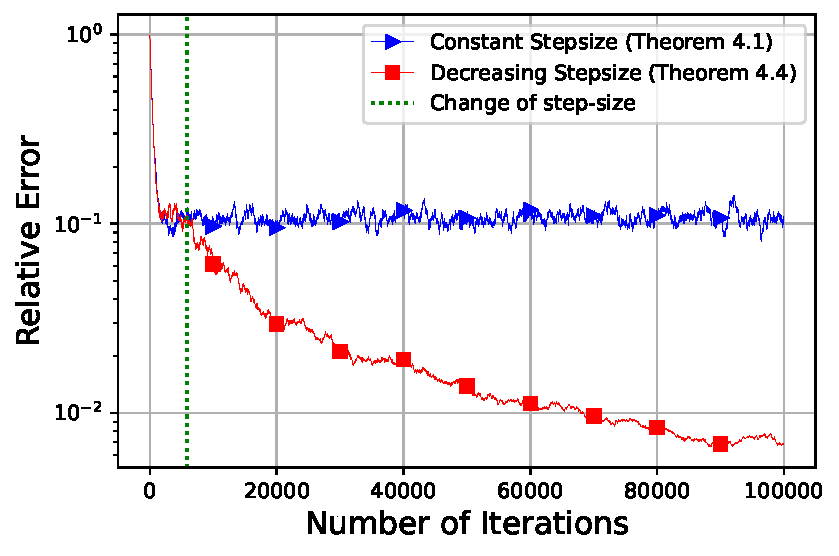
\includegraphics[width=0.49\textwidth]{Figures/Constant vs Switch Experiment 2 Final.pdf}
            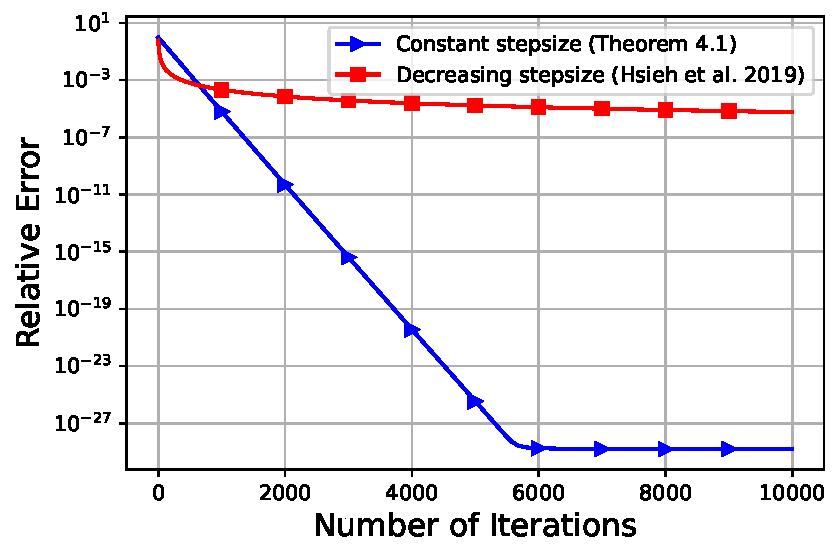
\includegraphics[width=0.49\textwidth]{Figures/Constant vs Hsieh on Interpolated Data Final.pdf}
            \caption{Comparison of \ref{eq:SPEGupdate} using our proposed step-size against decreasing step-size of \href{https://papers.nips.cc/paper_files/paper/2019/file/4625d8e31dad7d1c4c83399a6eb62f0c-Paper.pdf}{[11]} for solving \eqref{ansodna}. In the left plot, we use the switching step size, while in the right plot, we implement \ref{eq:SPEGupdate} with constant step size for the interpolated model ($\sigma_*^2=0$).}
            % \caption{Caption}
            % \label{fig:my_label}
        \end{figure}
        % \vspace{-1cm}
        \underline{\textbf{Importance Sampling}:}  \qquad  \qquad          \underline{\textbf{Weak Minty VIP}:}      
        \begin{figure}
            \centering
            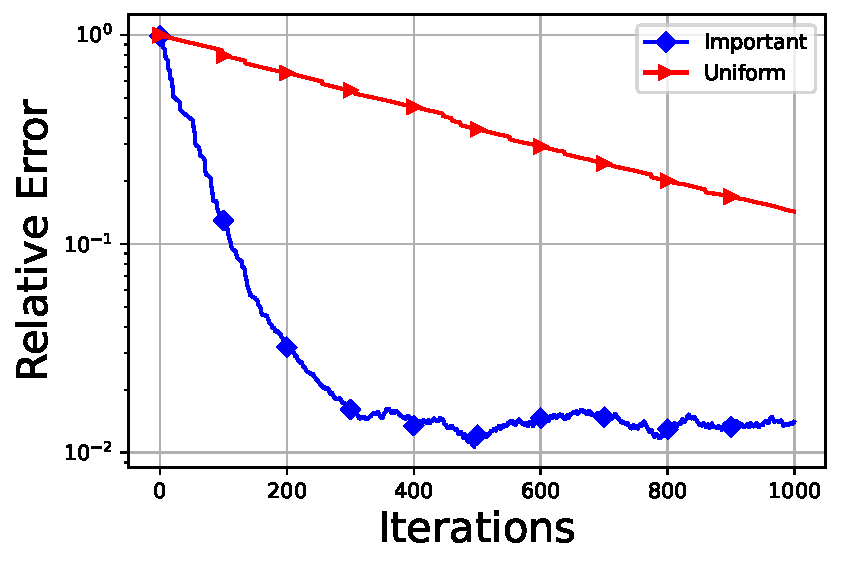
\includegraphics[width=0.49\textwidth]{Figures/Uniform vs Important Sampling with Lmax = 20 .pdf}
            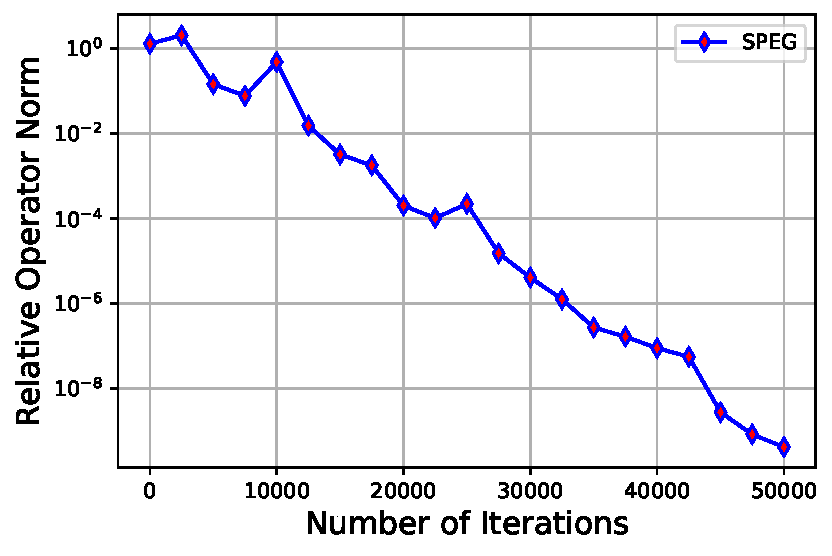
\includegraphics[width=0.49\textwidth]{Figures/SPEG_on_WMVI_w_rel_op_err_batchsize = 0.15.pdf}
            % \caption{Caption}
            % \label{fig:my_label}
            \caption{In the left plot, we demonstrate the advantage of using importance sampling over Uniform sampling for \ref{eq:SPEGupdate}. In the second plot, we implement \ref{eq:SPEGupdate} with our proposed step-sizes for solving a Weak Minty \ref{eq:VIP} of the form $\min_{x \in \mathbb{R}} \max_{y \in \mathbb{R}} \frac{1}{n} \sum_{i = 1}^n \xi_{i} xy + \frac{\zeta_i}{2}(x^2 - y^2)$.}
        \end{figure}
        % \vspace{-1cm}
        $\bullet$ Code to reproduce our result:\href{https://github.com/isayantan/Single-Call-Stochastic-Extragradient-Methods}{https://github.com/isayantan/Single-Call-Stochastic-Extragradient-Methods}.
        \end{block}		
		\end{column} % End of the top fourth column
  
  \end{columns}

\vspace{-1cm}
\begin{block}{References}
			\end{block}
\vspace{-3cm}
\begin{columns}[t,totalwidth=\twocolwid]

\begin{column}{\onecolwid}
\tiny{\begin{enumerate}[label={[\arabic*]}]
   \item G. Gidel, H. Berard, G. Vignoud, P. Vincent, and S. Lacoste-Julien. A variational inequality perspective on generative adversarial networks. ICLR, 2019.
   \item ] S. Sokota, R. D’Orazio, J. Z. Kolter, N. Loizou, M. Lanctot, I. Mitliagkas, N. Brown, and C. Kroer. A unified approach to reinforcement learning, quantal response equilibria, and two-player zero-sum games. ICLR, 2023.
   \item Y. Yu, T. Lin, E. V. Mazumdar, and M. Jordan. Fast distributionally robust learning with variance-reduced min-max optimization. In AISTATS, 2022.
   \item N. Loizou, H. Berard, G. Gidel, I. Mitliagkas, and S. Lacoste-Julien. Stochastic gradient descent-ascent and consensus optimization for smooth games: Convergence analysis under expected co-coercivity. NeurIPS, 2021.
   \item J. Diakonikolas, C. Daskalakis, and M. Jordan. Efficient methods for structured nonconvexnonconcave min-max optimization. AISTATS, 2021.
\end{enumerate}}
    
\end{column}

\begin{column}{\onecolwid}
\tiny{\begin{enumerate}[label={[\arabic*]}]
\setcounter{enumi}{5}
\item L. D. Popov. A modification of the arrow-hurwicz method for search of saddle points. Mathematical notes of the Academy of Sciences of the USSR, 1980.
\item G. M. Korpelevich. The extragradient method for finding saddle points and other problems. Matecon, 1976.
\item A. Böhm. Solving nonconvex-nonconcave min-max problems exhibiting weak minty solutions. TMLR 2022.
\item E. Gorbunov, A. Taylor, S. Horváth, and G. Gidel. Convergence of proximal point and extragradient-based methods beyond monotonicity: the case of negative comonotonicity. ICML, 2023.
\item E. Gorbunov, H. Berard, G. Gidel, and N. Loizou. Stochastic extragradient: General analysis and improved rates. AISTATS, 2022.
\item Y.-G. Hsieh, F. Iutzeler, J. Malick, and P. Mertikopoulos. On the convergence of single-call stochastic extra-gradient methods. NeurIPS, 2019.


\end{enumerate}}
    
\end{column}

\end{columns}
  
  \end{column}
		
  \end{columns}
	%----------------------------------------------------------------------------------------
	%	CONTACT INFORMATION
	%----------------------------------------------------------------------------------------
	
	\setbeamercolor{block alerted title}{fg=black,bg=YellowGreen} % Change the alert block title colors
	\setbeamercolor{block alerted body}{fg=black,bg=white} % Change the alert block body colors
	
	
	%----------------------------------------------------------------------------------------
	%	LOGOS
	%-----------------------------------6-----------------------------------------------------
	%\TPoptions{overlay = false}
	\begin{textblock*}{\onecolwid}(2cm,1cm)
		
\includegraphics[width=0.56\linewidth]{Figures/logoJHU.jpg}
	\end{textblock*}
	\begin{textblock*}{\onecolwid}(\paperwidth -16cm, 3cm)
		
\includegraphics[width=0.54\linewidth]{Figures/logoMBZUAI.png}
	\end{textblock*}
		%----------------------------------------------------------------------------------------
\end{frame} % End of the enclosing frame

\end{document}
